\documentclass[]{template/llncs}
\usepackage{url}
\usepackage{graphicx}
\usepackage{amsmath}
\usepackage{amsfonts}
\usepackage[linesnumbered,ruled,vlined]{algorithm2e}
\usepackage[
colorlinks = true,
linkcolor = black,
anchorcolor = black,
citecolor = black,
filecolor = black,
urlcolor = black
]{hyperref}
\usepackage{xeCJK} 
\setCJKmainfont{PingFangSC-Light}

\begin{document}
\bibliographystyle{unsrt}
\pagestyle{plain}

%
\title{ZKSwap:基于 ZK-Rollup的Layer2 代币Swap协议}

\author{L2 Lab}

\institute{
\email{dev@l2lab.org} \\
\vspace{0.5cm}
\today
}

\maketitle

%
\section{引言}

2019年以来,区块链行业发生了翻天覆地的变化,分布式金融 DeFi 正在快速崛起。各类链上资产在各种 DeFi 协议中,锁定的资产规模已突破100亿美金。随着链上资产的继续蓬勃发展和链下资产上链的不断推进,我们有理由相信 DeFi 协议锁定的资产规模将很快突破1000亿美金的市值。这些链上资产都有 快速、零摩擦、免信任实时兑换的需求,因此带动了 Uniswap \cite{uniswapofficial} 等新型兑换协议的崛起。

虽然以 Uniswap 为代表的新型 DEX 取得了很大的发展,但是依然有非常明确的缺点。第一:动辄几十美金的 Gas 费用,阻碍了新增用户进入;  第二:每一笔交易、每一个操作都需要等待至少一个区块确认,实时性差; 第三:受制于以太坊链上 TPS 的限制,Uniswap 每秒钟可以成交的交易次数和交易容量有明显的天花板。以上三点是目前所有 DEX 面临的痛点。

ZK-Rollup \cite{zkrollups} 是一种新型的 Layer-2 扩容方案,与 Plasma 等其他 Layer-2 扩容方案相比,ZK-Rollup 在安全性、经济性、TPS以及可用性方面都有巨大的优势,特别适合用于搭建Layer-2去中心化交易所。

ZKSwap (ZK-Rollup based Swap)是一套全新的基于 Zkrollup 技术的兑换协议,通过 Zk-Rollups 技术把所有的ERC20 token 转移到 Layer2 上,基于不断生成的零知识证明来保证 Layer1 和 Layer2 状态的一致性,从而让所有的兑换在 Layer2 上发生,可以做到零 Gas 费用的实时兑换(不再要等待一个区块确认时间),并且具备无限的拓展性,摆脱以太坊 TPS 和区块确认时间的限制,让 DEX 具备CEX (中心化交易所)般丝滑的体验,并同时实时掌控自己的资金安全。我们认为ZKSwap 就是未来的交易形态,必将对现有所有的 DEX 和 CEX 带来极大的变革。

目前大部分开发工作已经完成,我们将在10月初发布ZKSwap的兑换协议,后续我们将推动Layer-2 上面的DEX 兑换标准,使目前现有的 DEX,都可以无缝接入和使用 ZKSwap 突破性的兑换协议。


\section{技术基础}

\subsection{Uniswap v1 版本}
Uniswap\cite{uniswapv1} 是一套基于“固定乘积”自动化做市商机制的去中心化交易协议,由一系列部署在以太坊上的智能合约组成。用户可以通过提供一定比例的 ETH 和任意 ERC20 资产创建资金池,每个资金池都保存了一对资产,并为这两种资产的交易提供流动性。所有流动性的提供者会根据所提供流动性的比例分享交易量的 0.3\% 作为回报。在 uniswap 中,第一个流动性提供者需要设定资金池中两种资产的比例,自动做市商算法会保证每次交易前后两种资产的乘积保持恒定。以下简要介绍 uniswap 各项基本操作,帮助理解后文相关概念。

\subsubsection{创建资金池}

在 Uniswap 中,每个交易对有且只有一个资金池,一般由第一个流动性提供者创建。例如,流动性提供者创建了一个 ETH-ZKS 的资金池,随后可以开始添加流动性。初始存入的 ETH 数量为 $x_0$,存入的 ZKS 数量为 $y_0$,且 $x_0*y_0 = c_0$。其中,ZKS 是以太坊上任意 ERC-20 代币。

\subsubsection{流动性代币}

流动性提供者(Liquidity Provider,以下简称 LP)将获得对应资金池的流动性代币(Liquidity Provider Token,以下简称 LP Token),用来代表LP占目前资金池的份额。LP Token 是一种符合 ERC-20 标准代币,可以在不移除资金池流动性的情况下进行传输。每个资金池都有一种对应的 LP Token。上述初始 LP 可以获得 $n_0 = \sqrt{(x_0*y_0)} - MIN\_LIQUIDITY$ 个 LP Token。其中,由于LP Token 的总量将在后续计算中作为分母被用到,因此在首次添加流动性时, 系统会把 $MIN\_LIQUIDITY$ 作为 LP Token 最小预留量,发送到 0x0 地址,防止 LP Token 总量变为零。

以下假设在任意时刻 $i$,资金池中有 $x_i$ 个 ETH,$y_i$ 个 ZKS 代币,它们的乘积常量为 $c_i = x_i *y_i$,发行的 LP Token 总量为 $n_i$。其中,$i = 0,1,2,……$

\subsubsection{添加流动性}

用户可以根据当前资金池中代币的比例,以同等比例添加流动性,并获得 LP Token。假设新的 LP 向流动性池中注入 $X$ 个 ETH 和 $Y$ 个 ZKS,注入时必须保证 $X/Y = x_i/y_i$。该 LP 可以获得合约增发的 $N = n_i*X/x_i$ 个 LP Token。增加流动性之后,资金池的 reserve 将更新为 $x_{i+1}*y_{i+1} =  (x_i+X)*(y_i+Y) = c_{i+1}$。LP Token 的总量为 $n_{i+1} = n_i + N$。

\subsubsection{减少流动性}

 LP 可以通过在流动性池合约中销毁 LP Token 来减少流动性,并从资金池中取回对应份额的 ETH 和 ZKS 代币。假设 LP 销毁的 LP Token 数量为 N’,则 LP 可取回的 ETH 数量为 $X’ = x_i*N’/n_i$,可取回的 ZKS 代币的数量为 $Y’ = y_i*N’/n_i$。移除流动性后,资金池的reserve 将更新为 $x_{i+1}*y_{i+1} = (x_i - X’)*(y_i - Y’) = c_{i+1}$。LP Token 总量更新为 $n_{i+1} = n_i - N'$。值得注意的是,由于 LP 在添加流动性和移除流动性时资金池的 reserve 可能不同,因此 LP 存入和取出的币的数量和比例都可能发生变化。

\subsubsection{Swap 交易}

资金池创建并注入流动性后,持有 ETH 或 ZKS 的用户就可以开始在资金池中进行 Swap,用 ETH 兑换 ZKS,或者用 ZKS 兑换 ETH。这里以用 ETH 兑换 ZKS 为例。用户向资金池中转入 $m$ 个 ETH,资金池中 ETH 将变为 $x_{i+1} = x_i + m,$用户可以对应获得 $y_{i+1}$ 个 ZKS 代币。根据 uniswap 的 AMM 算法,在扣除 $0.003m$ 的手续费后,应保持 $(x_{i+1} - 0.003m)*y_{i+1} = x_i*y_i$。因此,用户将获得 $y_{i+1} = (x_i*y_i)/(x_{i+1} - 0.003m)$ 个 ZKS 代币。手续费会在交易后自动加入资金池的 reserve,因此交易后整个资金池的reserve 变为 $x_{i+1}*y_{i+1} = c_{i+1} > c_i$由于没有新的 LP Token 生成或销毁,LP Token 的总量保持不变,即 $n_{i+1} = n_i$。这意味着所有 LP 的份额不变,但每单位份额对应的资金池 reserve 总量增加了。


\subsection{Uniswap v2 版本}
Uniswap v1 实现了基本的 AMM 交易所功能,但也存在一些问题。但由于其合约是不可升级的,开发团队为了修复这一问题,又重新实现了一版 Uniswap v2 \cite{uniswapv2},其基本功能和 Uniswap v1 一致,但增加了一些新特性,包括:

\begin{itemize}
	\item 可以直接创建两种 ERC-20 代币的交易对,而不需要像 uniswap v1 一样需要通过 ETH 作为中间媒介来间接进行两者的交易;
	\item 更加合理的价格预言机,利用区块第一笔交易前一笔交易价格的随机性,使价格不容易被操控;
	\item 闪电兑换(Flash Swap),用户可以先获得目标代币,后续再完成swap;或者可以在规定时间内归还代币,从而不触发swap过程,这相当于可以借用资金池中的代币;
	\item 资金池中原本交易收取的 0.3\% 手续费可以分为两部分,其中 0.25\% 仍用于手续费,另外 0.05\% 被发送到预先设定的地址,作为预留的协议手续费,可用作不同用途;
\end{itemize}

这些新增特性增加了uniswap 的实用性,本文所述的 ZKSwap 的交易特性与 uniswap v2 保持一致。

\subsection{ZK-Rollup 和 zkSync}
ZK-Rollups 是近年来比较流行的 Layer-2 扩容解决方案,其基本思想是通过把大量交易聚合,链上验证证明的方式达到扩容的目的。ZK-Rollups 通过智能合约来解析和验证这些聚合的交易,并利用零知识证明技术把聚合交易的证明上链,从而减少了链上需要存储的数据。所有资金本身都锁定在智能合约中,而大部分的计算和存储都放在链下。
zkSync\cite{zksync} 是 ZK-Rollups 的一个实现,目前其 v1 版本已经在以太坊主网部署。其基本的工作原理如下:
\begin{itemize}
	\item 用户把签好名的交易提交给 Validator;
	\item Validator 把一段时间内收到的多笔交易执行 roll up 操作,合并为一个区块,并把更新后的合约状态树的根哈希,以及状态更新对应的 SNARK 证明发送到链上合约中。这个SNARK 可以证明新状态确实是这一系列交易作用在旧状态上的结果;
	\item 另外,validator 还会把每笔交易对应的状态增量 ∆ 发送到链上,这使得任何人都可以重新构建出每一笔交易后的状态;
	\item 上述的SNARK证明和状态增量∆都需要经过链上合约的验证,从而证明所有交易的合法性以及区块数据的可用性。
\end{itemize}

由于 SNARK 验证的 Gas 消耗远小于验证大量单笔交易的 Gas 消耗总和,且把完整状态存在链下也比存在链上要便宜,因此 ZK-Rollup 在理论上可以实现对以太坊主网 100~200 倍的扩容,同时显著降低 Gas 消耗。
ZK-Rollup 的安全性几乎和对应 Layer-1 的安全性保持一致,因为:

\begin{itemize}
	\item Validator 无法篡改状态,也无法挪用任何 Layer-2 的资金,因为所有状态的改变都需要对应的证明,无法伪造;且私钥始终掌握在用户手中;
	\item 由于链上存储了交易状态的增量和相关证明,即使 Validator 停止工作,用户也可以从链上数据恢复出每一笔交易,并取回锁定的 Token;
	\item 用户不需要保持在线,因为不需要存储任何额外数据。
\end{itemize}

zkSync 目前支持三种操作:

\begin{itemize}
	\item Deposit,存币:把 Layer-1 中的 Token 转移到 zkSync Layer-2;
	\item Withdraw,取币:从 Layer-2 中取回账户的 Token,并发送到 Layer-1 的账户;
	\item Transfer,转账:在 Layer-2 上实现 Token 的转账,无需手续费。
\end{itemize}

\section{ZKSwap 去中心化 Swap 协议}

本项目实现一种基于 ZK-Rollup 技术的 Layer-2 AMM 去中心化交易协议 ZKSwap,在 Layer-2 上实现了uniswap 的所有功能,在保证去中心化交易的核心价值的同时,实现实时交易,把 Uniswap 的 TPS(每秒可以处理的交易数量)提升了多个数量级,同时交易的过程几乎不需要消耗任何 Gas 费用。

\subsection{ZKSwap 系统框架}

ZKSwap 系统由链上智能合约,链下ZKSwap Server,零知识证明系统和前端用户界面组成。

\begin{figure}[htbp]
\centering
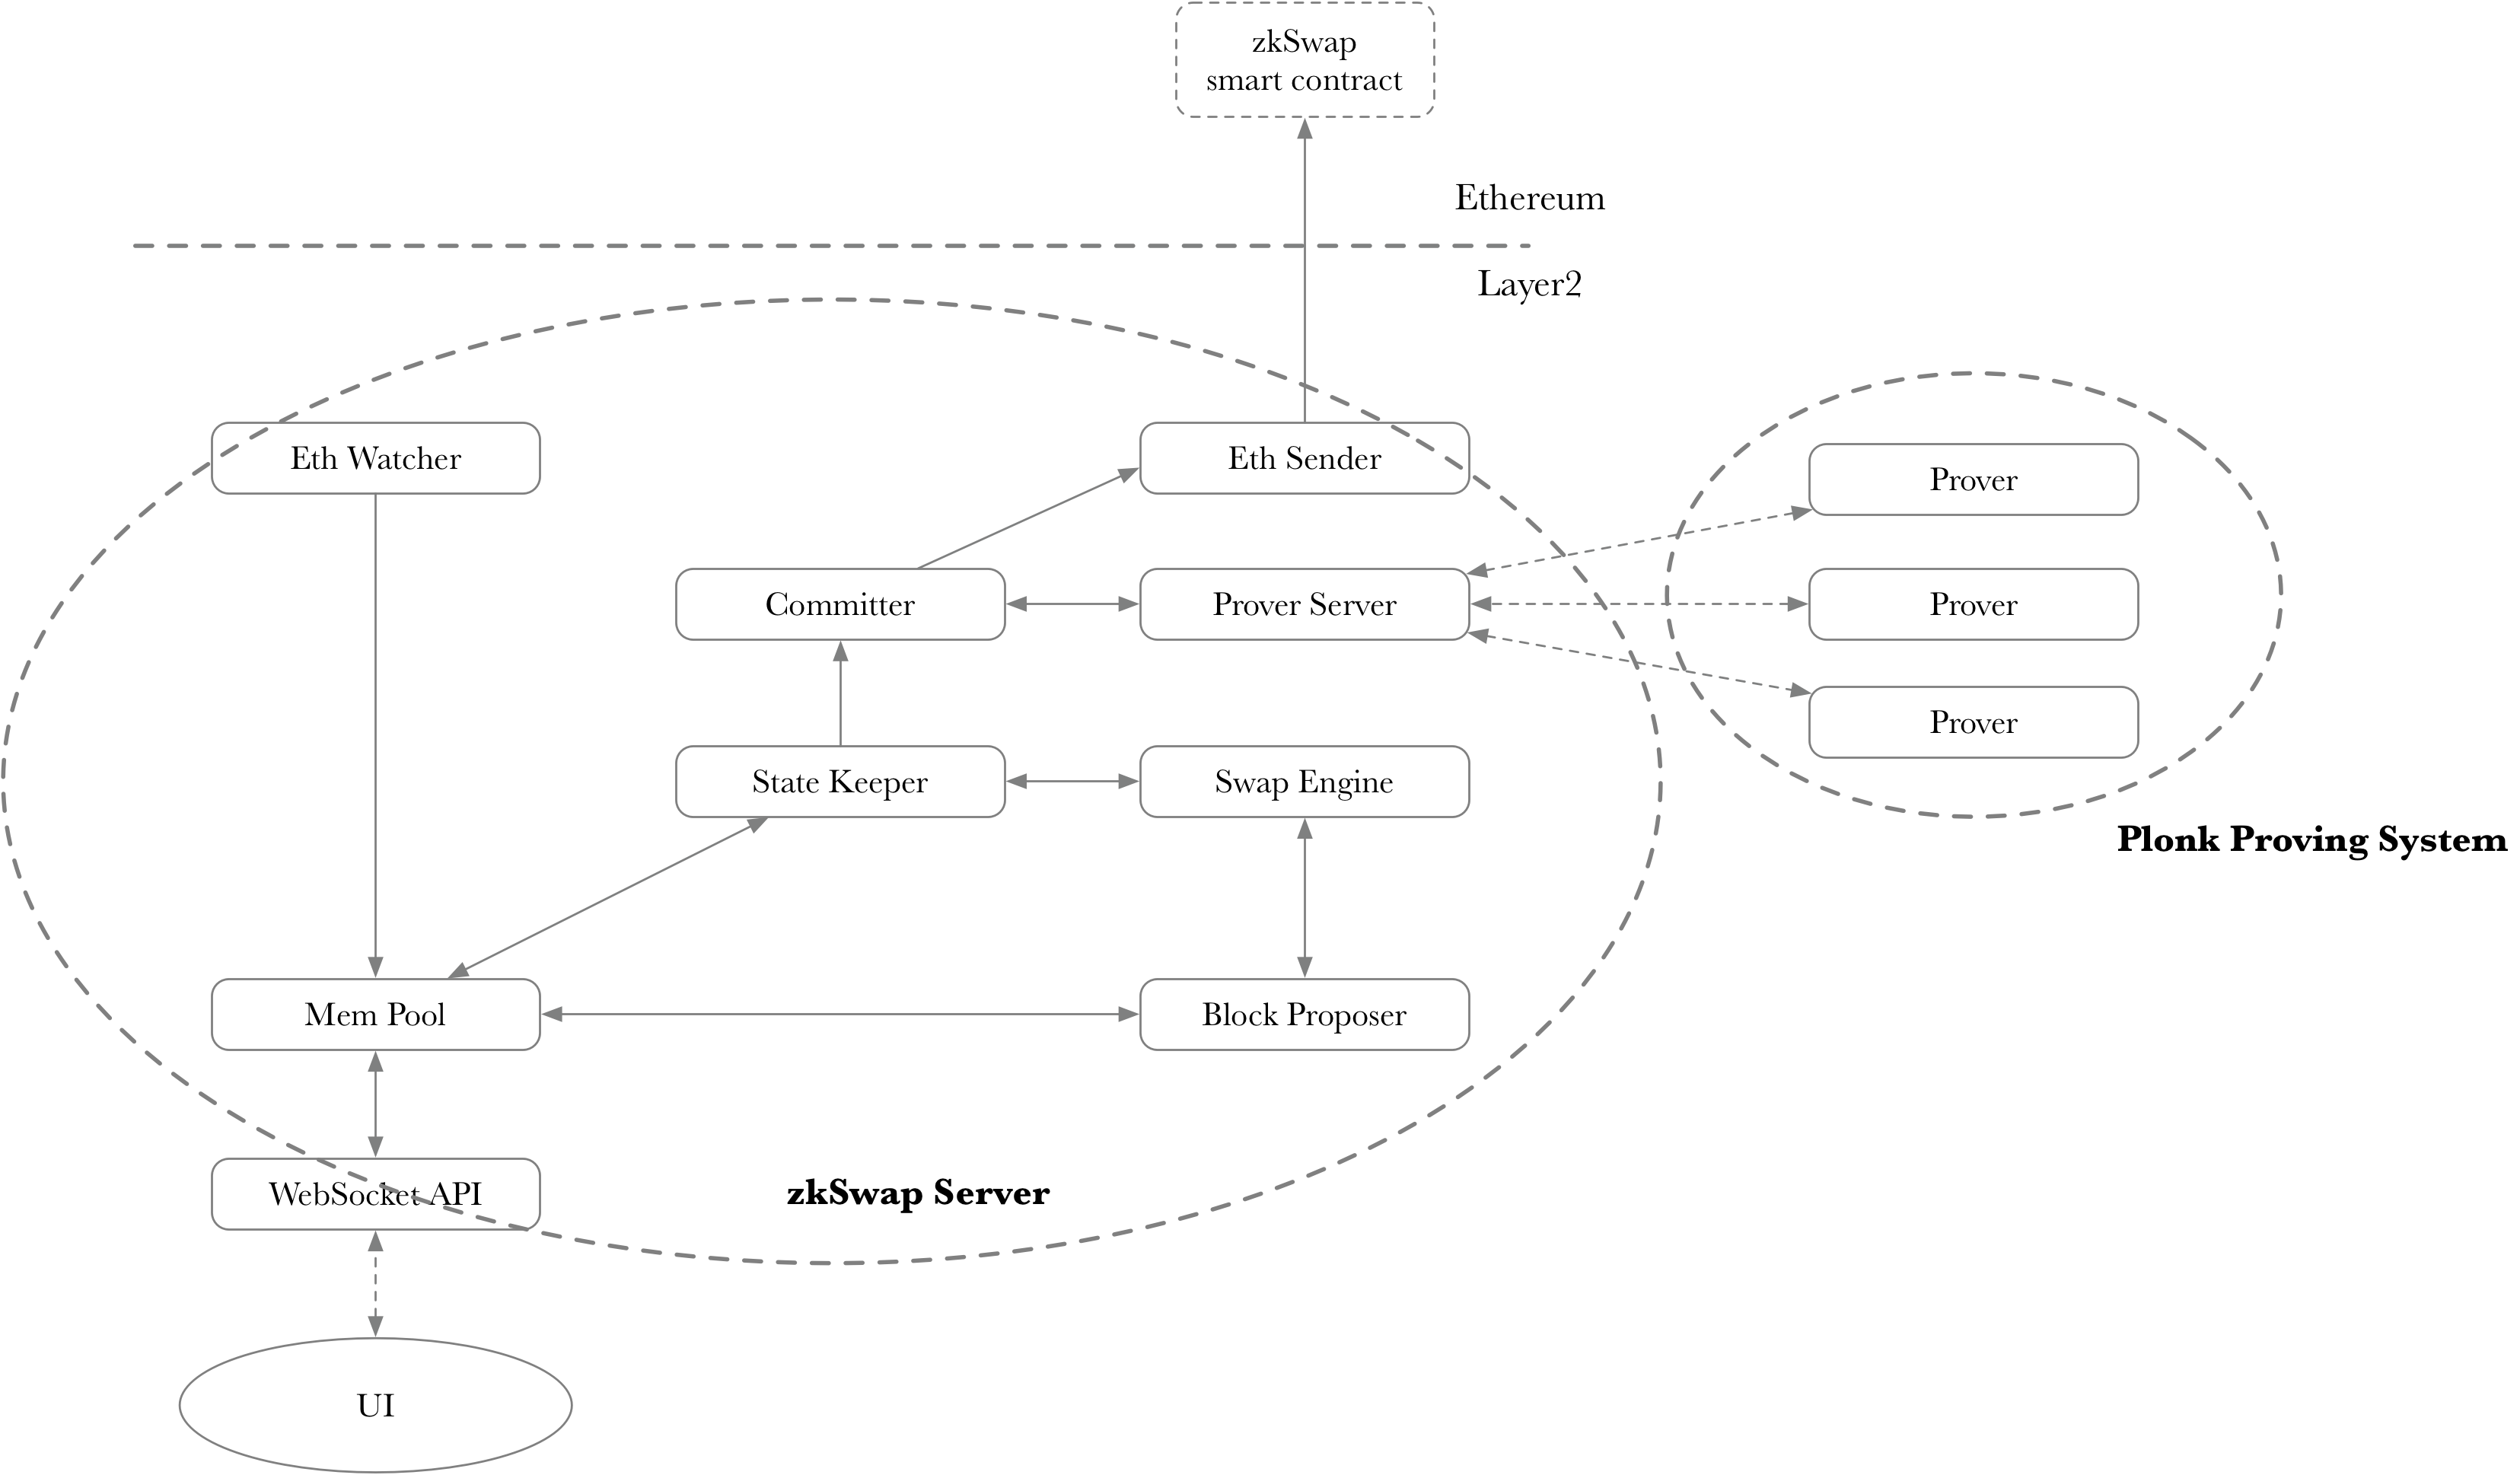
\includegraphics[width=0.9\columnwidth]{figure/arch}
\caption{系统架构}
\label{fig:arch}
\end{figure}

\subsubsection{ZKSwap 智能合约}

ZKSwap 会在以太坊区块链上部署一系列智能合约,用于存储用户存入的代币,同时需要记录和验证Layer-2的状态更新和相关证明,是连接链上和链下的关键枢纽。

\subsubsection{ZKSwap Layer-2 服务端}

ZKSwap 服务端是在链下实际处理所有交易的模块。ZKSwap 服务端可以通过 WebSocket 接口和用户发生交互,同时还可以监听以太坊区块链上的交易。所有合法的交易请求将被放入 ZKSwap 内存池中,最终由 Swap Engine 负责处理。内存池中的交易类型和上一节中 Uniswap 所有操作类型保持一致。Block proposer 对交易进行 Rollup,生成新区块,并由 State Keeper 更新 Layer-2 中所有代币的状态。State Keeper 会把状态发送给 Commiter,后者负责与Prove server 通信,获得对应交易的证明,并最终将状态和对应的 SNARK 证明通过 Ethererum sender 发送到链上的 ZKSwap 智能合约。

\subsubsection{Plonk 零知识证明系}

ZKSwap 的零知识证明系统采用分布式架构,并采用最新的零知识证明算法 PLONK\cite{cryptoeprint:2019:953} 生成证明。Prove server支持多个Prover。多个Prover 主动查询 Prove server 中的证明任务,生成证明后发回 Prove server。PLONK 的全局 trust setup只需要生成一次,电路规模在一定范围内的应用都可复用,极大地降低了零知识证明的使用门槛。

\subsection{ZKSwap 状态树}

\begin{figure}[htbp]
\centering
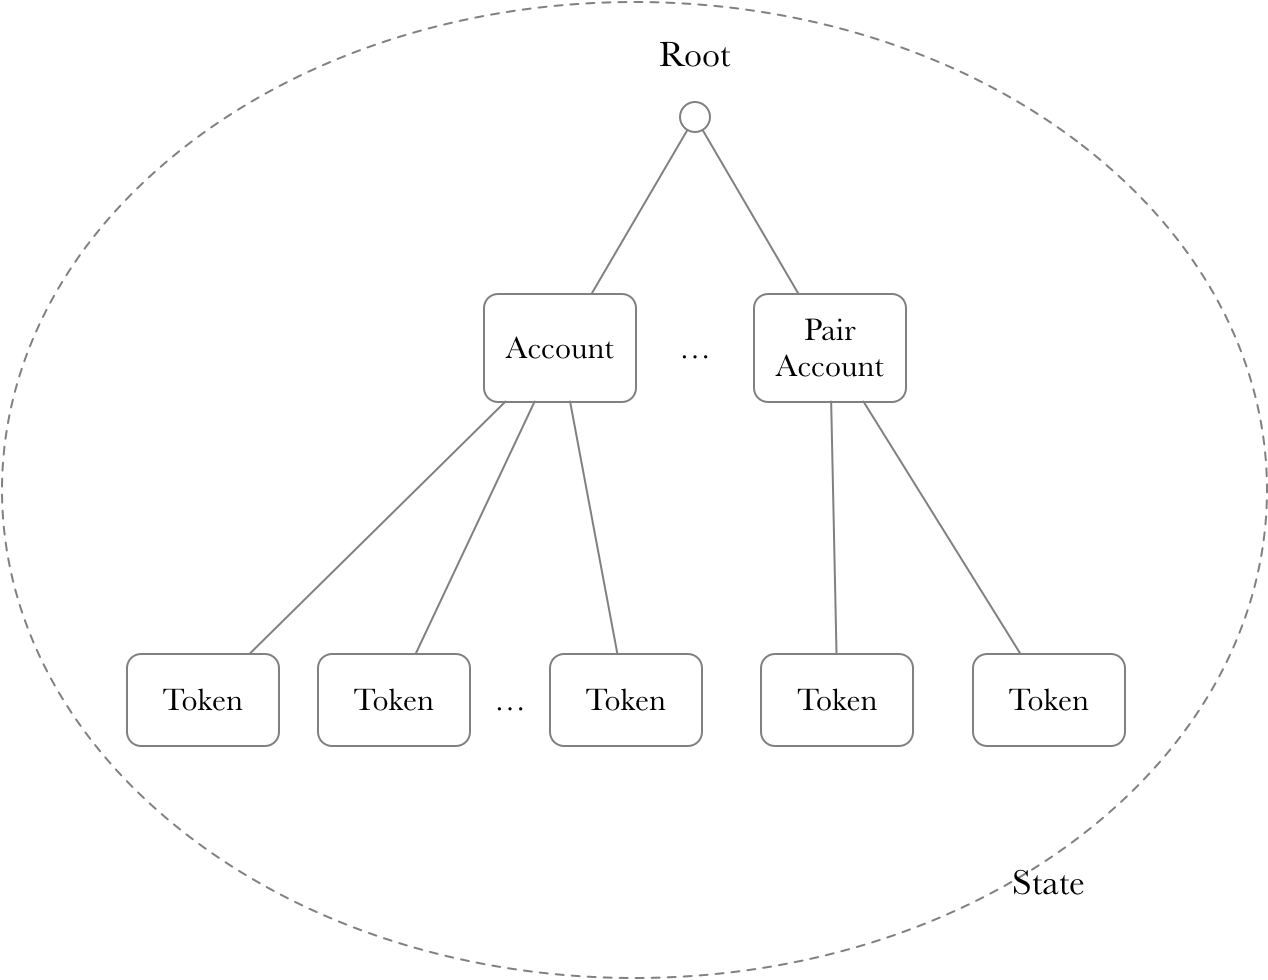
\includegraphics[width=0.9\columnwidth]{figure/state}
\caption{状态树}
\label{fig:state}
\end{figure}

ZKSwap 系统的状态树记录了当前系统中所有账户的余额状态。ZKSwap 的状态树是一棵高度为 34的默克尔树。根节点 Root 的子节点为系统中所有账户节点(24层)。账户节点分为两种类型:

\begin{itemize}
	\item 普通账户节点,用于记录账户内所有 Token 的状态。普通账户节点可以有任意多个叶子节点(10层),每个叶子节点都代表一种类型的 Token 及其数量;同一账户下的 Token 类型不可重复;
	\item Pair 账户节点,用于记录 ZKSwap 中某个交易对资金池的状态。Pair 账户节点只包含两个叶子节点,每个叶子节点代表该资金池中一种 Token 的余额和类型。
\end{itemize}

ZKSwap 中交易的过程实际就是状态树更新的过程。下面介绍 ZKSwap 中所有交易类型和对应的状态变化。

\subsection{存币(Deposit )}

\begin{figure}[htbp]
\centering
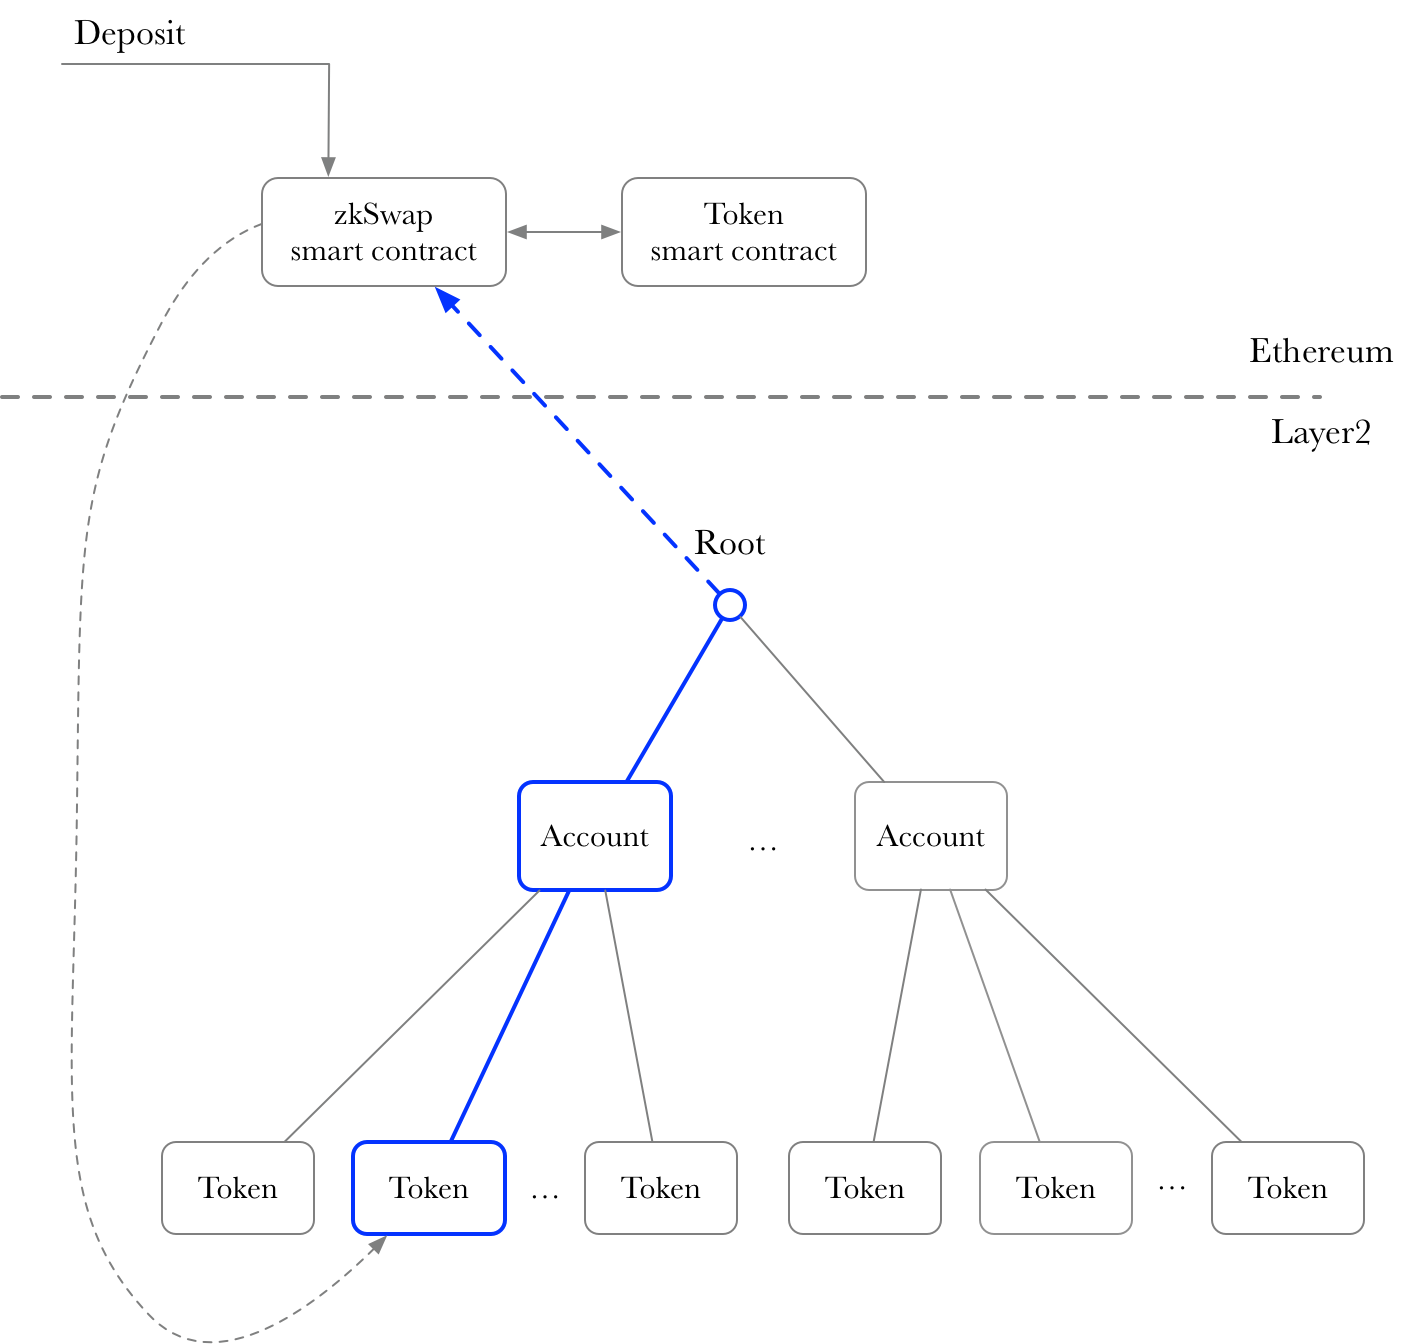
\includegraphics[width=0.9\columnwidth]{figure/deposit}
\caption{Deposit}
\label{fig:deposit}
\end{figure}

Deposit 是指用户把以太坊链上的代币存入 ZKSwap 合约,使其可以在 Layer-2 中使用的过程。Deposit 操作由用户从链上发起。当 ZKSwap Server 监听到用户在链上将 Token 转入 ZKSwap 智能合约的交易后,会根据交易详情更新状态树。首先,根据交易所属的账户找到对应的 Account,并根据 Deposit 的金额更新 Account 下对应 Token 的状态。若该 Account 下没有对应 Token 的叶子节点,首先需要创建该 Token 对应的叶子节点,再进行状态更新。叶子节点的状态更新完成后,根节点的哈希也会随之更新。

更新后的状态树根节点哈希会和 Deposit 交易的 SNARK 证明一起被发送到链上的 ZKSwap 合约中。

\subsection{取币(Withdraw)}

\begin{figure}[htbp]
\centering
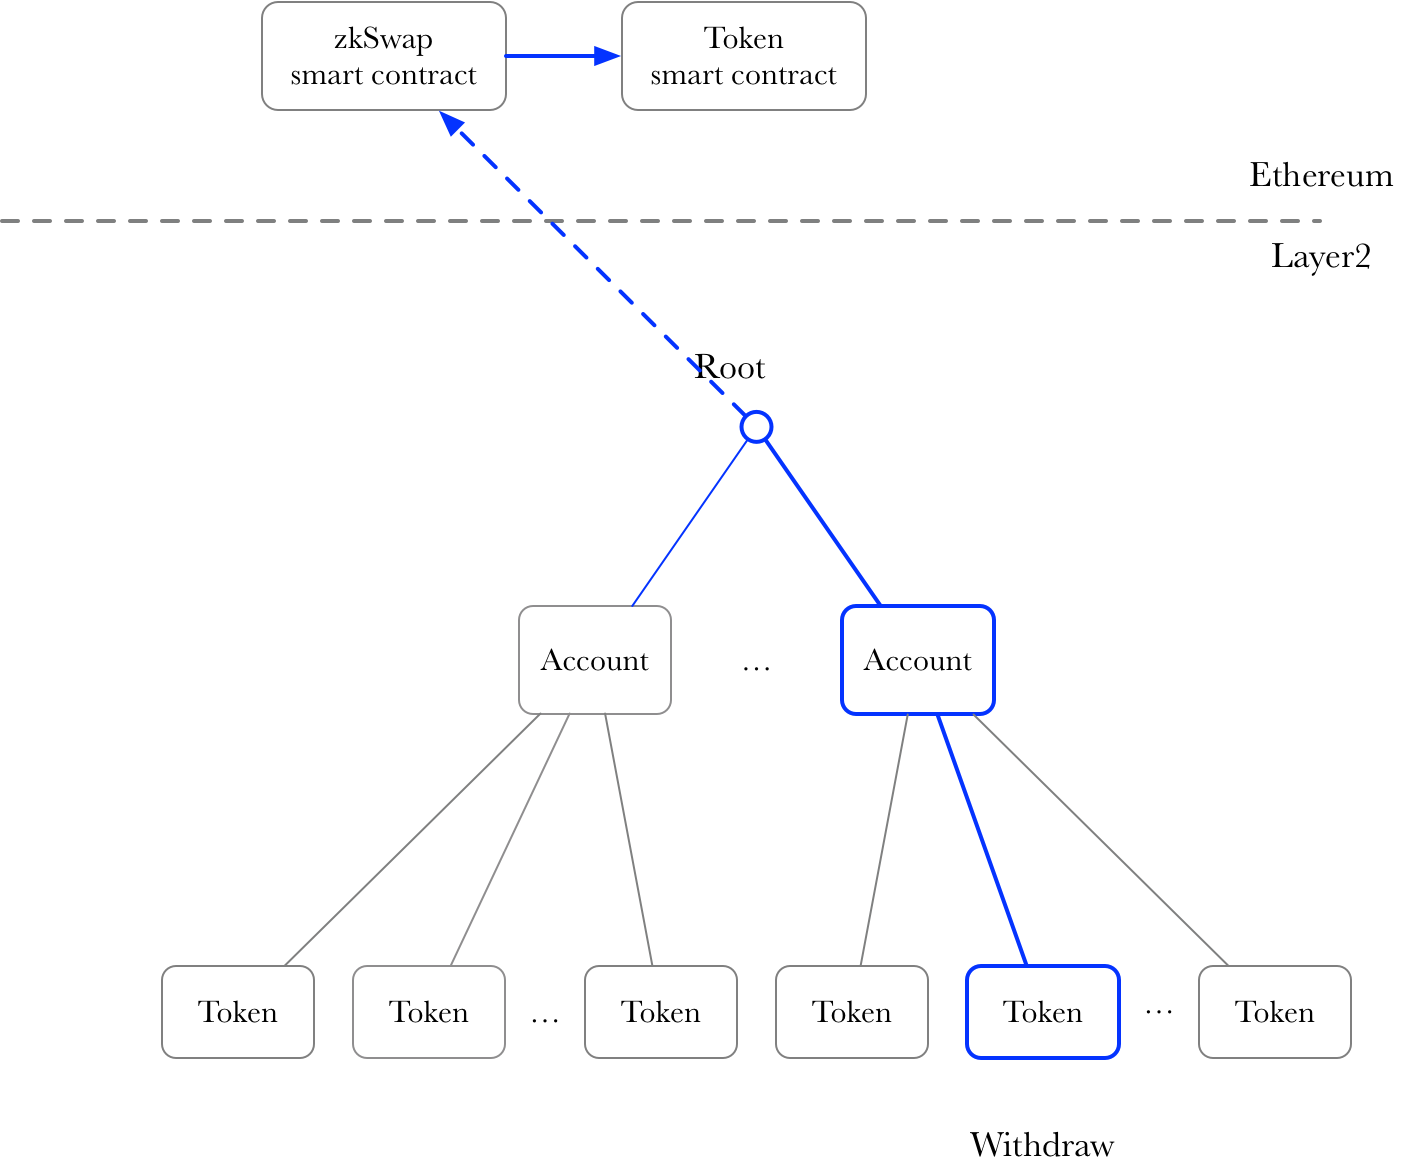
\includegraphics[width=0.9\columnwidth]{figure/withdraw}
\caption{Withdraw}
\label{fig:withdraw}
\end{figure}

Withdraw 是指用户从 Layer-2 中将 Token 提出,并从 ZKSwap 合约中解锁,发到对应 Layer-1 账户的过程。Withdraw 操作由用户从 Layer-2 发起,ZKSwap server 在收到用户对某一 Token 的提币请求后,会更新对应账户下对应 Token 的状态,并把更新后的状态树根节点哈希和 Withdraw 操作应用的证明发送到链上 ZKSwap 合约。合约验证通过后会把合约中锁定的对应 Token 发送到对应链上账户。

\subsection{转账(Transfer)}

\begin{figure}[htbp]
\centering
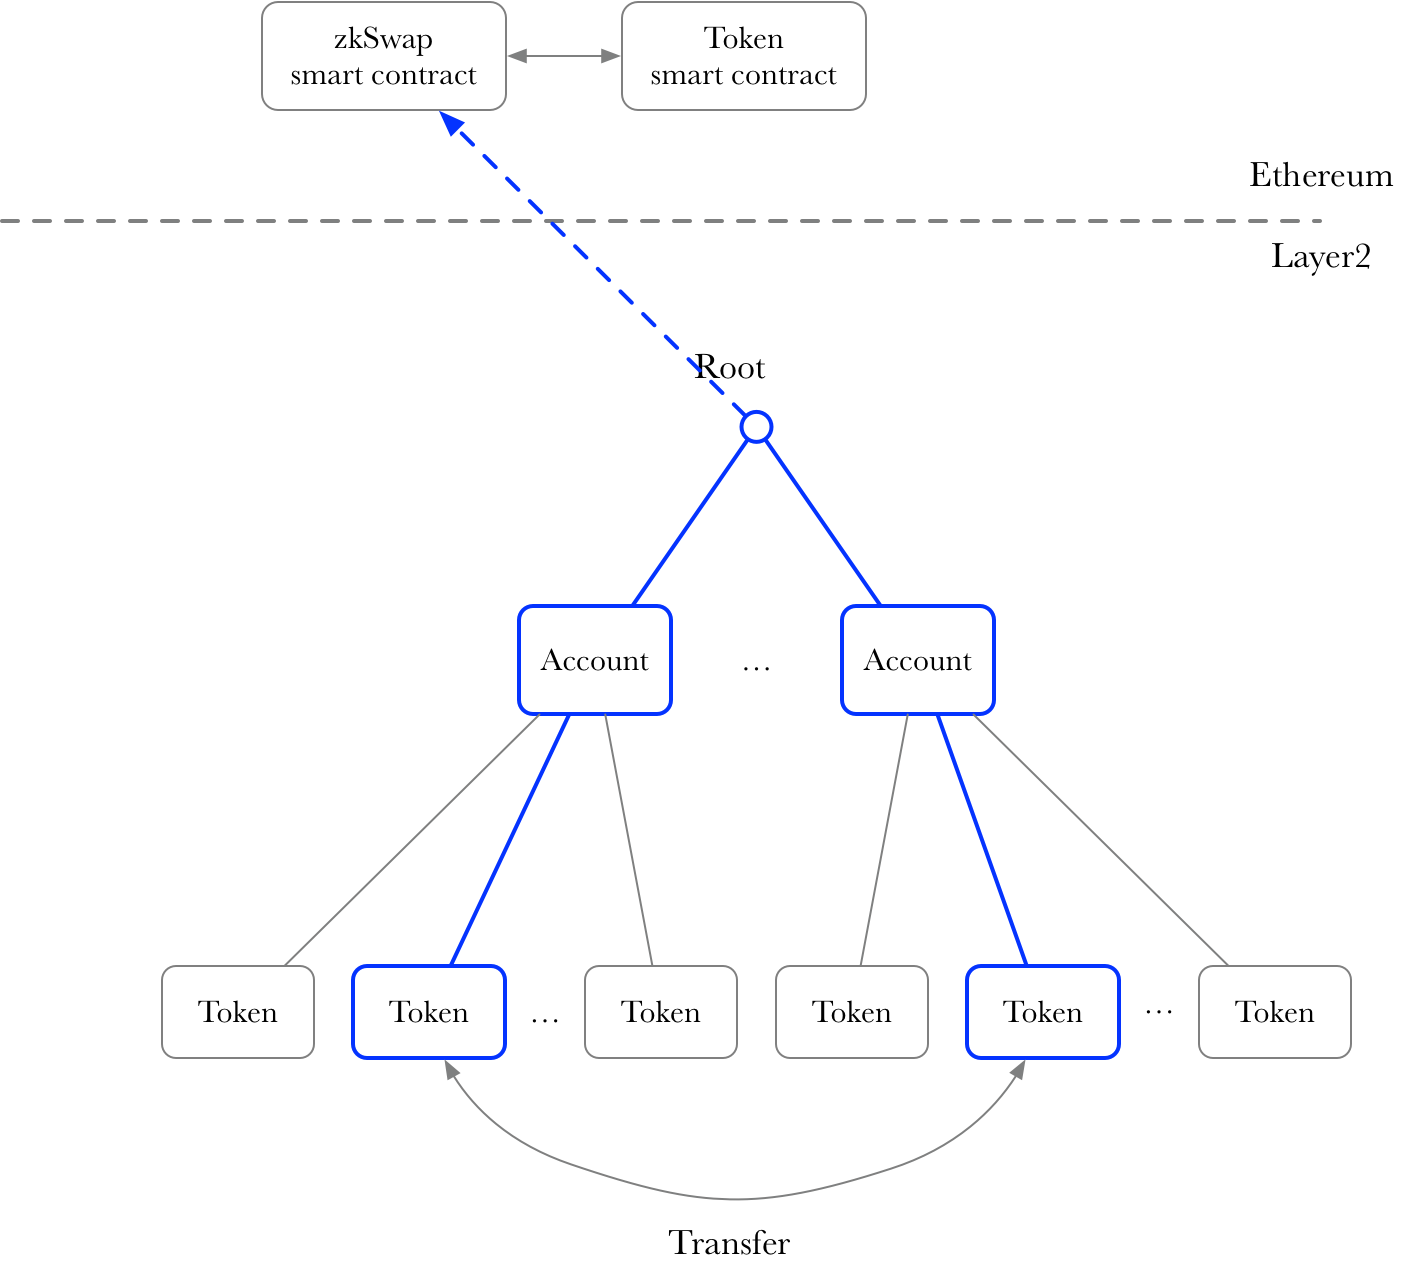
\includegraphics[width=0.9\columnwidth]{figure/transfer}
\caption{Transfer}
\label{fig:transfer}
\end{figure}

Transfer 是指用户在 ZKSwap Layer-2 把某种 Token 发送给另一用户的过程。Transfer 由用户在 Layer-2 发起。当 ZKSwap Server 收到 Transfer 请求后,会根据请求详情找到对应的收发账户,并根据发送金额更新收发双方账户下该 Token 的状态。状态树根节点哈希也会随之更新,并和 Transfer 操作对应的 SNARK 证明一起被发送到 ZKSwap 链上合约。Transfer 不会改变链上对应 Token 的状态,因为 Token 仍然锁定在 ZKSwap 合约中,并没有在链上发生转移。

\pagebreak

\subsection{增加流动性(Create Liquidity)}

\begin{figure}[htbp]
\centering
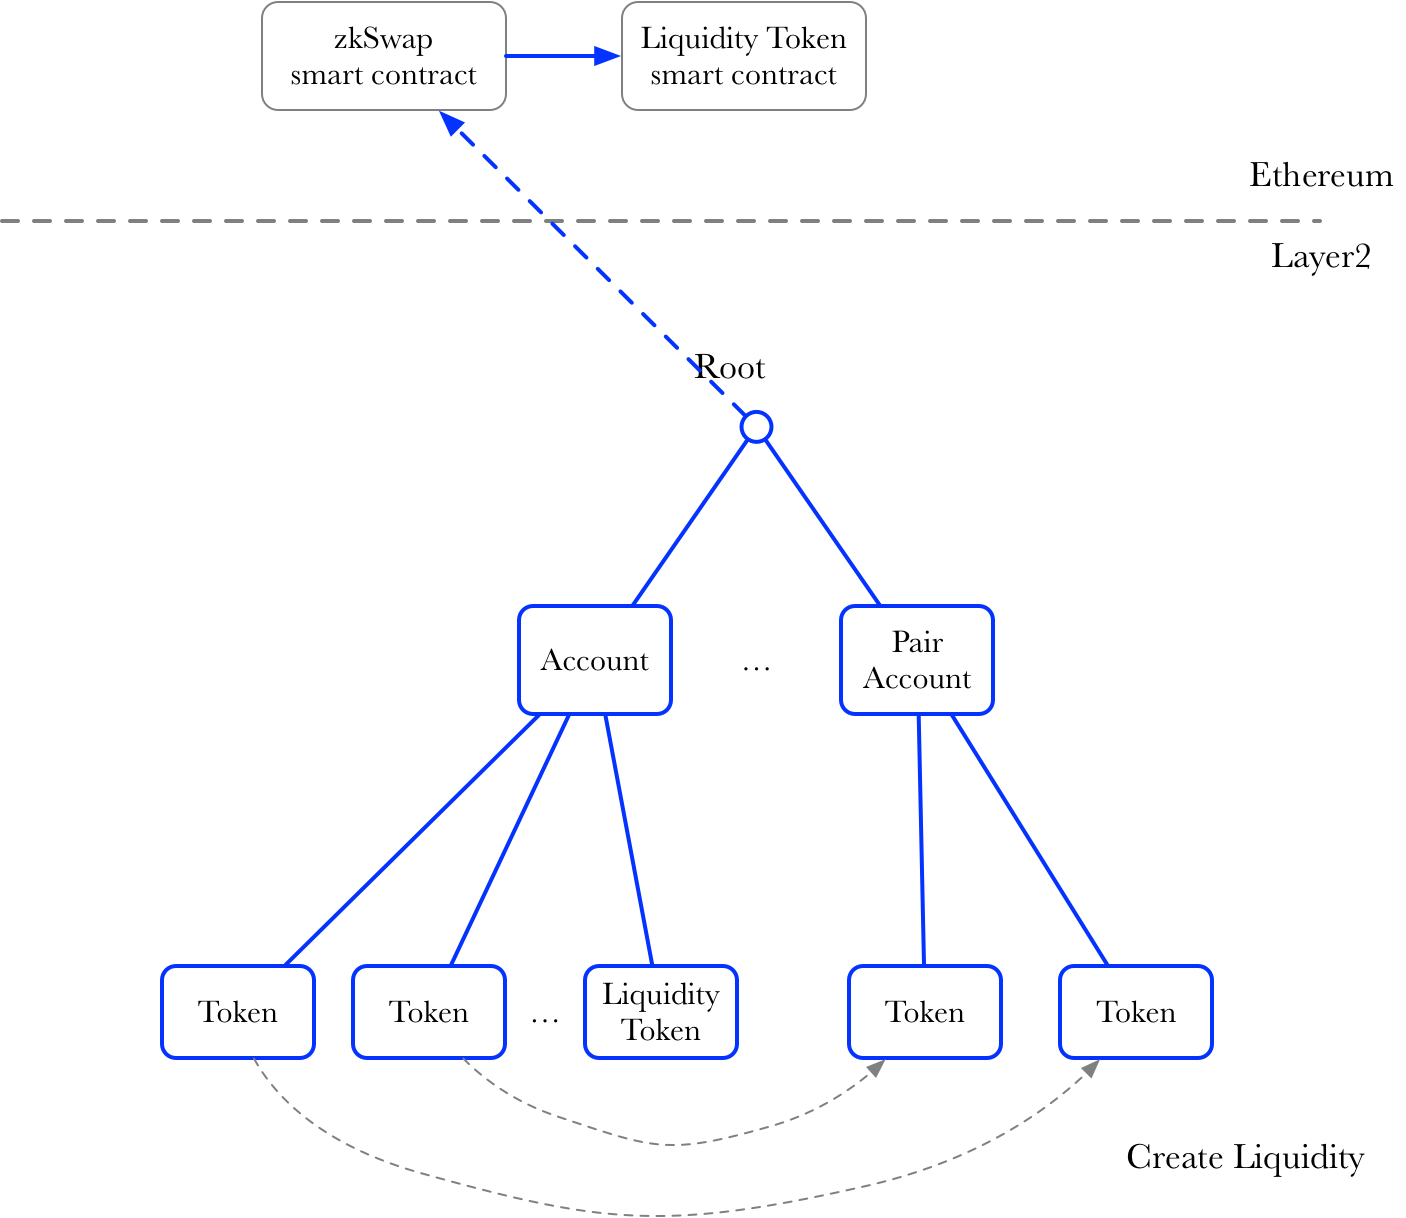
\includegraphics[width=0.9\columnwidth]{figure/create_liquidity}
\caption{Create Liquidity}
\label{fig:create_liquidity}
\end{figure}

Create liquidity 是指用户在 Layer-2 完成创建或增加流动性的操作,其定义和 uniswap 保持一致。Create liquidity 由用户在 Layer-2 发起,当 ZKSwap server 收到用户创建某一对 Token 流动性的请求后,首先需要找到对应的发起人 Account 和这一对 Token 的 Pair Account(若 Pair Account 不存在,需要先创建 Pair 资金池);然后把 Account 下两种 Token 按照 AMM 算法规定的比例要求 Transfer 到 Pair Account 下;同时系统会计算出用户可以获得的 LP Token 数量,并更新流动性提供者 Account 下对应的 LP Token 状态。所有状态更新完成后,状态树的根节点哈希将会和 Create Liquidity 对应的证明一起被发送到链上的 ZKSwap 合约。首次创建的 LP token 需要由 ZKSwap 合约在链上部署对应 LP Token 的合约。

\pagebreak


\subsection{减少流动性(Remove Liquidity)}

\begin{figure}[htbp]
\centering
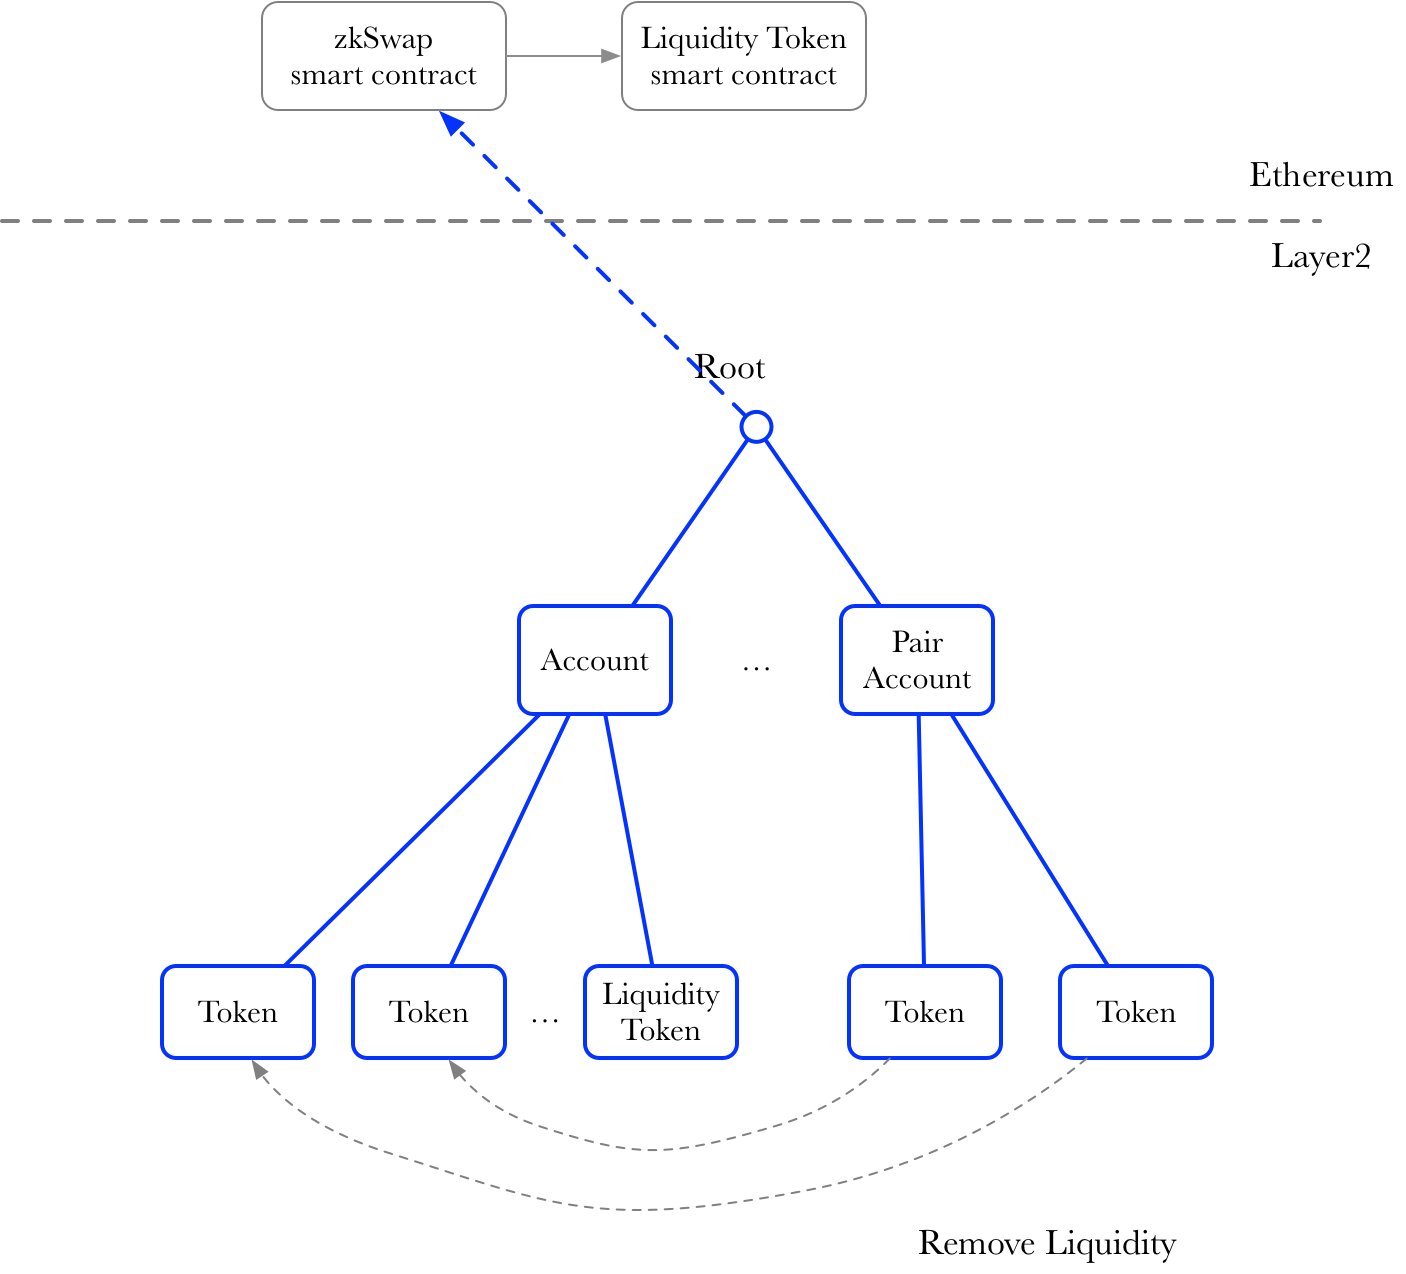
\includegraphics[width=0.9\columnwidth]{figure/remove_liquidity}
\caption{Remove Liquidity}
\label{fig:remove_liquidity}
\end{figure}

Remove Liquidity 是指用户从 Layer-2 的某一 Pair 资金池中销毁 LP Token,并在 Layer-2 中取回相应比例的两种 Token 的过程。Remove Liquidity 由用户在 Layer-2 发起,当 ZKSwap Server 收到用户 Remove Liquidity 请求时,首先会找到对应 Account,销毁 Account 下对应数量的 Liquidity Token;接着会将 Liquidity Token 对应的 Pair Account 下的两种 Token 按照比例 Transfer 给销毁 Liquidity Token 的 Account。操作完成后状态树会做相应更新,根节点哈希和对应的 Remove Liquidity 操作的证明将被发送到链上的 ZKSwap 合约。

\pagebreak


\subsection{Swap 交易}

\begin{figure}[htbp]
\centering
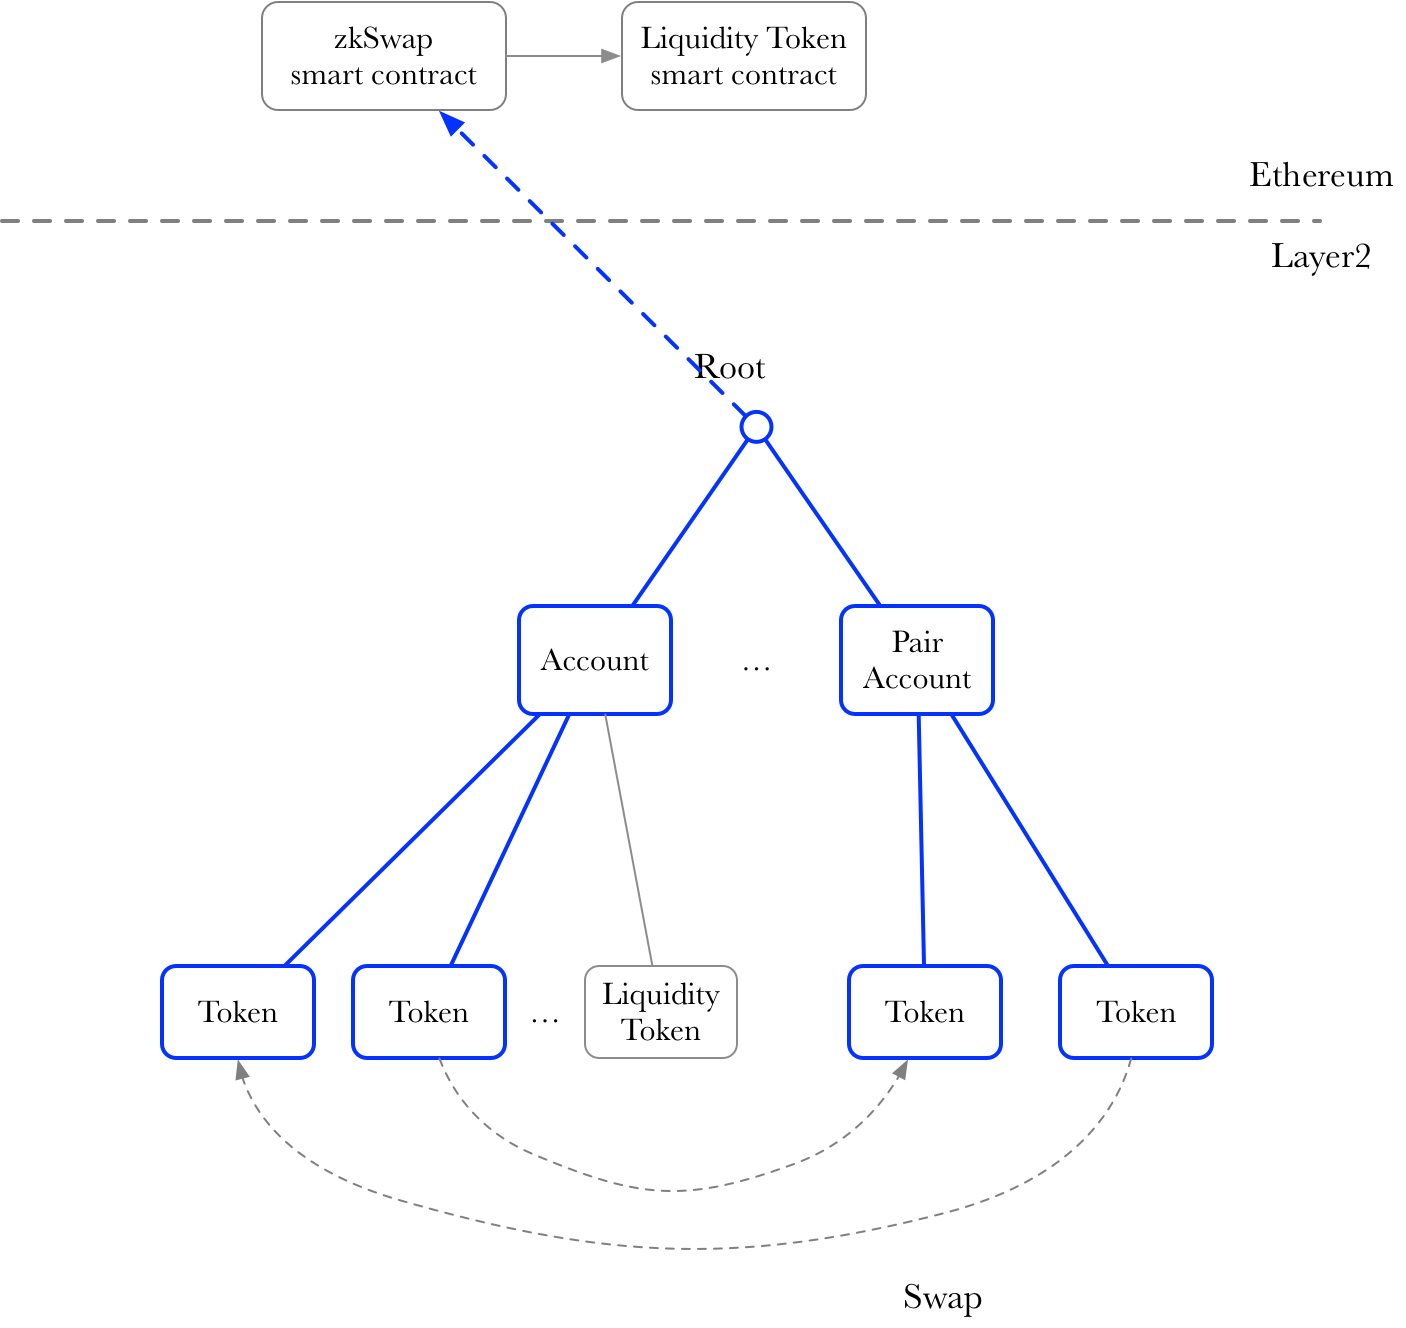
\includegraphics[width=0.9\columnwidth]{figure/swap}
\caption{Swap 交易}
\label{fig:swap}
\end{figure}

Swap 是指用户在 Layer-2 的资金池中完成交易的过程。假设用户需要在包含 TokenA -TokenB Pair Token 的资金池中进行 Swap 交易。用户首先从 Layer-2 将自己 Account 下的 TokenA 发送到对应的 Pair Account,ZKSwap 会根据 AMM 算法计算用户可以获得的 TokenB 的数量并发送给用户。状态树随之更新,ZKSwap Server会将更新后的状态树根节点哈希以及 Swap 操作对应的证明发送到链上的 ZKSwap 合约。Swap 交易不会改变链上 Token 的状态,因为 Token 本身仍然锁定在 ZKSwap 合约中。

\subsection{提取流动性(Withdraw Liquidity)}

\begin{figure}[htbp]
\centering
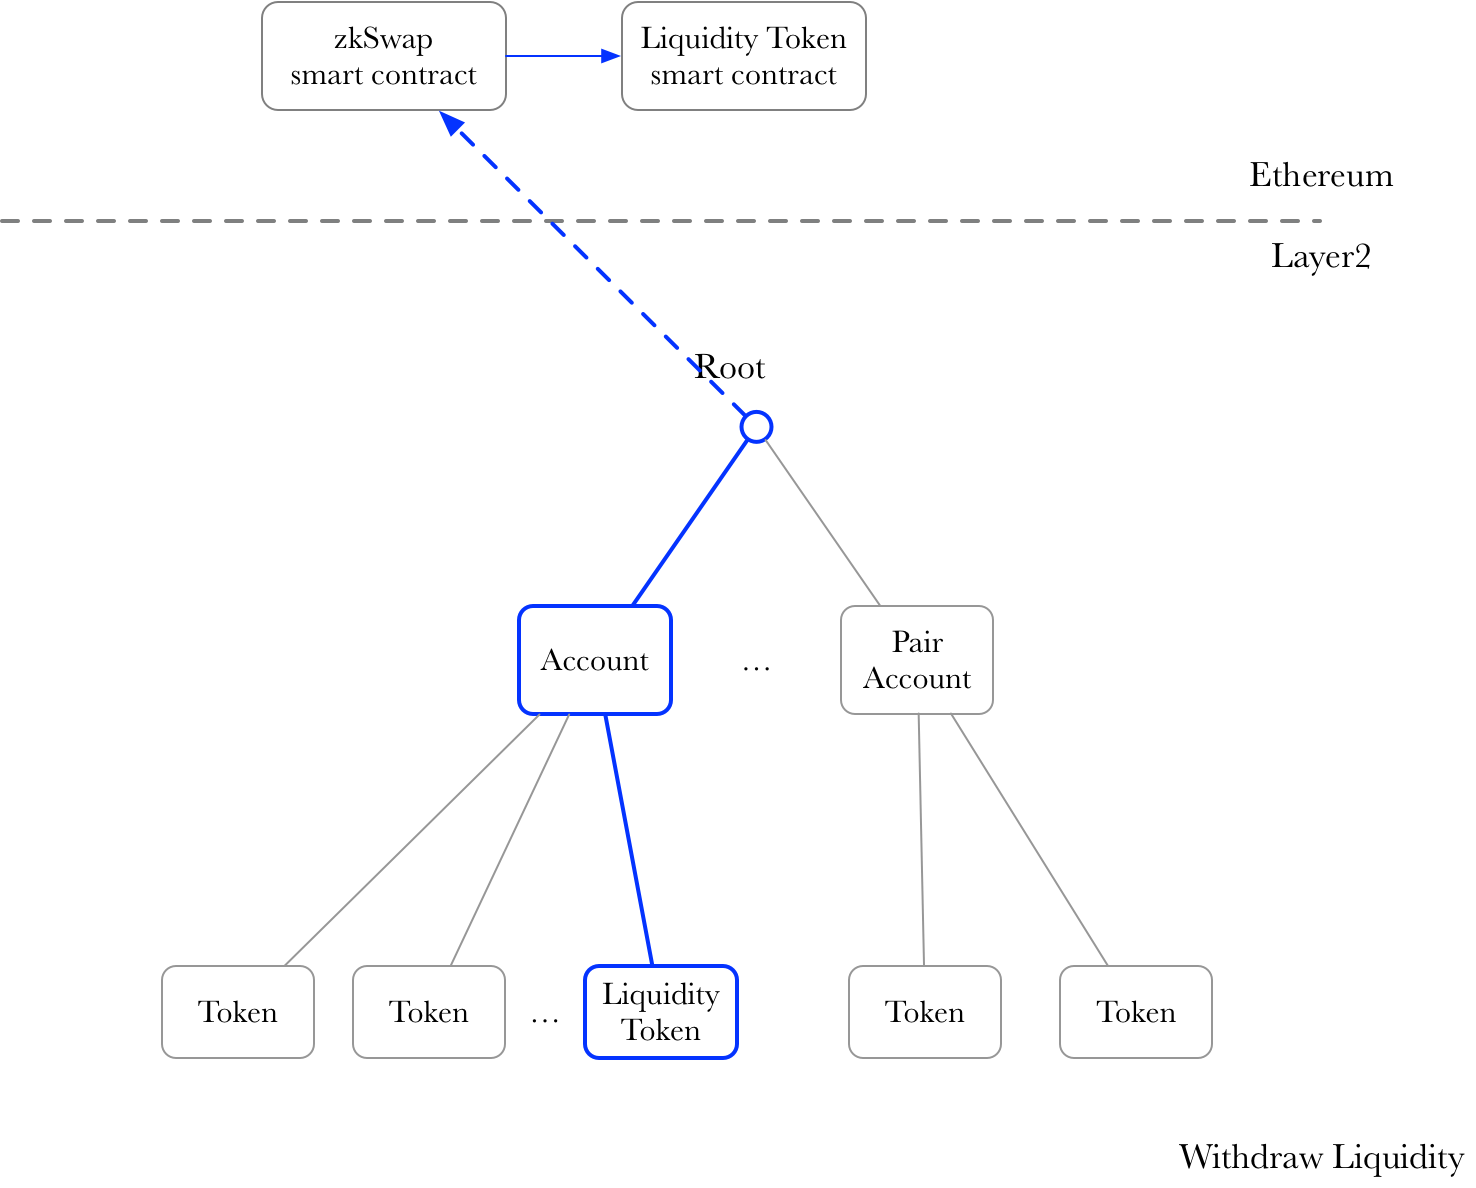
\includegraphics[width=0.9\columnwidth]{figure/withdraw_liquidity}
\caption{Withdraw Liquidity}
\label{fig:withdraw_liquidity}
\end{figure}

Withdraw Liquidity 是指用户从 Layer-2 账户中的 Liquidity Token 提取到 Layer-1 的过程。Withdraw Liquidity 在 Layer-2 的发起过程和状态更新与上述普通的 Withdraw 完全一致,但在 Layer-1 中产生的结果不同。ZKSwap 合约收到 Withdraw Liquidity 请求后,会自动触发 Liquidity Token 的 mint 操作,在 Layer-1 中创造出额外的 Liquidity Token,并发送给指定账户。


\section{总结与展望}

ZKSwap 利用 ZK-Rollup 技术,在 Layer-2 实现了 Uniswap 的完整功能,是一套去中心化的 Layer-2 代币 AMM 自动化做市商 Swap 协议。ZKSwap 协议可无限扩展,支持超高 TPS,且流动性提供者和用户不需要支付高昂的 gas 费用,并且具备实时交易性,用户不再需要等待区块确认,就可以在Layer2 上面完成极速的交易,极大降低了DEX的使用门槛,对现在所有的DEX 和CEX 都带来了巨大变革。

ZKSwap 由 L2 Lab 支持开发。在未来,L2 Lab 将继续推动 Layer-2 协议层的发展,结合 ZKSwap、Layer-2 隐私稳定币等一系列 Layer-2 基础协议,打造完整的 Layer-2 DeFi 生态。

通过打造用户体验极佳的的 Layer-2 协议标准,L2 Lab 致力于推动区块链行业的范式转换,让Layer-1 成为清结算的根基,Layer-2 成为连接区块链应用和 Layer-3 的桥梁和出入口。我们会致力于推动让所有的区块链应用都运行在没有任何限制的 Layer-3 的世界。
我们会致力于让ZKSwap 成为DEX中最好用的产品,时机成熟的时候,也会推出流动性挖矿计划和 DAO 计划,助力分布式金融 DeFi 的崛起,一起引领区块链应用的范式变革。


\bibliographystyle{template/splncs04}
\bibliography{zkswap.bib}

\end{document}